%*******************************************************************
%   Project Name: BracU Thesis Template
%   Prepared by: Ayesha Abed Library, Brac University
%   
%   "Predicting a T20 Cricket Match Result While The Match is in Progress", this thesis was 
%   submitted to BracU on 23 August, 2015 by Fahad Munir, Md. Kamrul Hasan, Sakib Ahmed, Sultan Md. Quraish
%   Authors have given full consent to use their thesis as a sample to develop a Thesis Template using LaTex 
%   PLEASE KEEP ALL FILES IN THEIR DESIGNATED FOLDERS
%*******************************************************************
% Project Structure:
% appendix: Contains “appendix.txt” files.
% bibliography: Contains “references.bib” file.
% chapters: Contains “chapter.txt” files. For every chapter, create separate “chapter_[1,2,3..].txt” files.
% core: This folder will contain following files:
%     declaration.txt
%     approval.txt
%     ethics_statement.txt
%     abstract.txt
%     dedication.txt
%     acknowledgement.txt
%     titlepage.txt
% images:Contains all images files. 
% main.txt
%     This is the main.txt file. All the packages and environment variable are declared in main.txt. All others .txt files are referred from this file.
%
% If you have any questions or concerns about the latex template, please feel free to visit Ayesha Abed Library.
%*******************************************************************

\documentclass[Times,12pt,oneside,openany,print,index]{report}
\usepackage[a4paper,width=150mm,top=25mm,bottom=25mm]{geometry}
\usepackage[english]{babel}
\usepackage[utf8]{inputenc}
\usepackage{csquotes} % Provides advanced facilities for in-line and display quotations
\usepackage{amsmath} % TO use mathematical equations 
\pagestyle{plain} % Just a plain page number. For more http://www.emerson.emory.edu/services/latex/latex_129.html
\usepackage{luacode}
\usepackage{graphicx} % to use the graphicx package
\graphicspath{/images} % Path to Image files 
\usepackage{caption} % To use caption with figure and images
\usepackage{array} % The array environment is used to make a table of information, with column alignment (left, center, or right) and optional vertical lines separating the columns

\usepackage[nottoc]{tocbibind} % The tocbibind package can be used to add the ToC and/or bibliography and/or the index etc., to the Table of Contents listing

\usepackage[normalem]{ulem} % The ulem package provides various types of underlining that can stretch between words and be broken across lines.

\usepackage{hyperref} % Provides LaTeX the ability to create hyperlinks within the document.
\hypersetup{
    colorlinks=true,
    linkcolor=black,
    filecolor=magenta,      
    urlcolor=black,
    citecolor=black,
}
\urlstyle{same}

\setlength{\parindent}{0em} % To control Indentation of paragraphs 

\usepackage{nomencl} % The nomenclature package can be used to generate and format a nomenclature using MakeIndex.
\renewcommand{\nompreamble}{The next list describes several symbols \& abbreviation that will be later used within the body of the document}
\makenomenclature

\usepackage[backend=biber,style=ieee,sorting=ynt]{biblatex} % for more plz click https://www.overleaf.com/learn/latex/Biblatex_citation_styles
\addbibresource{bibliography/references.bib} % Imports bibliography file

\let\cleardoublepage=\clearpage % removes unwanted doublepages

\begin{document}
% \input{student_info.tex} % Add title page
\thispagestyle{empty} % removes page number from title page
\directlua{dofile("core/script.lua")}
\newcommand*{\studentoneid}{\directlua{student_1_id()}}
\newcommand*{\studentonename}{\directlua{student_1_name()}}
\newcommand*{\studenttwoid}{\directlua{student_2_id()}}
\newcommand*{\studenttwoname}{\directlua{student_2_name()}}
\newcommand*{\studentthreeid}{\directlua{student_3_id()}}
\newcommand*{\studentthreename}{\directlua{student_3_name()}}
\newcommand*{\studentfourid}{\directlua{student_4_id()}}
\newcommand*{\studentfourname}{\directlua{student_4_name()}}
% \newcommand*{\studentfiveid}{\directlua{student_5_id()}}
\newcommand*{\studentfivename}{\directlua{student_5_name()}}
\newcommand*{\studentonecolor}{\directlua{student_1_color()}}
\newcommand*{\studenttwocolor}{\directlua{student_2_color()}}
\newcommand*{\studentthreecolor}{\directlua{student_3_color()}}
\newcommand*{\studentfourcolor}{\directlua{student_4_color()}}
% \newcommand*{\studentfivecolor}{\directlua{student_5_color()}}

\begin{titlepage}
\renewcommand*{\thepage}{Title} % Change page number in PDF
    \begin{center} 
        \vspace*{3cm} % For creating Vertical Blank Space
        
        {\fontsize{16pt}{22pt}\selectfont{Deep Learning and NLP-Based Cardiac Risk Prediction \\ Using ECG and EHR Data}
        } 
        
        \vspace{1.5cm}
        
        \text{by}
        
        \vspace{0.5cm}
            \color{\studentonecolor}
        	\studentonename\\\studentoneid\\
        	\color{\studenttwocolor}
	        \studenttwoname\\\studenttwoid\\
	        \color{\studentthreecolor}
	        \studentthreename\\\studentthreeid\\
	        \color{\studentfourcolor}
	        \studentfourname\\\studentfourid\\
	        % \color{\studentfivecolor}
	        % \studentfivename\\\studentfiveid\\ %comment out the student that does not belong to group.
            \color{black}
        \vspace{1.5cm}
        
        	A thesis submitted to the Department of Computer Science and Engineering\\
            in partial fulfillment of the requirements for the degree of\\
            B.Sc. in Computer Science

        
        \vspace{2.5cm}
        
    		Department of Computer Science and Engineering\\
            Brac University\\
            October 2024
        
        \vspace{3cm}
        
    		\copyright\ 2024. Brac University\\
            All rights reserved.
    
    \end{center}

\end{titlepage} % Add title page
\cleardoublepage

\pagenumbering{roman} % Roman numbers to be use all pages before Chapter 1

%*******************************************************************
% TOC = Table of Contents
% The hyperref makes Title page No. 1 entry in the TOC
% In order to properly link  all section in TOC "phantomsection" command used
%  see below link for details on "addcontentsline"
% http://www.emerson.emory.edu/services/latex/latex_162.html
% "input" command to add files
% "Ethics Statement" & "Dedication" page are Optional; you may omit this two page if you want
% Please do not change the order of listings in TOC
%*******************************************************************
\phantomsection
\addcontentsline{toc}{chapter}{Declaration}
% Following command is used to create grouped signature line for Four Authors
\newcommand*\wildcard[2][6cm]{\vspace{1cm}\parbox{#1}{\hrulefill\par#2}} 

% A "parbox{}{}" is a box whose contents are created in paragraph mode. 
% "hrulefill{} to change thickness of underline"

\section*{Declaration}

It is hereby declared that

\begin{enumerate} % begin{enumerate} function to create numbered list
  \item The thesis submitted is my/our own original work while completing degree at Brac University.
  \item The thesis does not contain material previously published or written by a third party, except where this is appropriately cited through full and accurate referencing.
  \item The thesis does not contain material which has been accepted, or submitted, for any other degree or diploma at a university or other institution.
  \item We have acknowledged all main sources of help.
\end{enumerate}

\vspace{1cm}
\textbf{Student’s Full Name \& Signature:} % Testbf{} for Bold
\vspace{.5cm}

% CROP the signatures with minimum height possible. The width will always be resized to 6cm.
\begin{center}
    \begin{tabular}[b]{@{} p{6cm} @{}}
        
\includegraphics[width=6cm]{images/signatures/tahmid.jpg} \\
        \hline
        \centerline{\studentonename}
        \centerline{\studentoneid}
    \end{tabular}
    % Remove the following 7 lines if there's no second author.
    \hspace{2.5cm} %horizontal space added to create a gap between the two signatures in the same line
    \begin{tabular}[b]{@{} p{6cm} @{}}
        
\includegraphics[width=6cm]{images/signatures/emon.jpg} \\
        \hline
        \centerline{\studenttwoname}
        \centerline{\studenttwoid}
    \end{tabular} \\ %this double backslash is to create a new signature in the next line
    % Remove the following 6 lines if there's no third author.
    \begin{tabular}[b]{@{} p{6cm} @{}}
        
\includegraphics[width=6cm]{images/signatures/Mehedi.jpg} \\
        \hline
        \centerline{\studentthreename}
        \centerline{\studentthreeid}
    \end{tabular}
    % Remove the following 7 lines if there's no fourth author.
    \hspace{2.5cm}
    \begin{tabular}[b]{@{} p{6cm} @{}}
        
\includegraphics[width=6cm]{images/signatures/nuclear.jpg} \\
        \hline
        \centerline{\studentfourname}
        \centerline{\studentfourid}
    \end{tabular} \\
    % Remove the following 6 lines if there's no fifth author.
 
\end{center}


\pagebreak







\phantomsection
\addcontentsline{toc}{chapter}{Approval}
\section*{Approval}

The thesis/project titled “Deep Learning and NLP-Based Cardiac Risk Prediction Using ECG and EHR Data” submitted by 
\begin{enumerate}
\color{\studentonecolor}
  \item \studentonename (\studentoneid)
  \color{\studenttwocolor}
  \item \studenttwoname (\studenttwoid)
  \color{\studentthreecolor}
  \item \studentthreename (\studentthreeid)
  \color{\studentfourcolor}
  \item \studentfourname (\studentfourid)
%   \color{\studentfivecolor}
%    \item \studentfivename (\studentfiveid)
   \color{black}
\end{enumerate}

Of Summer, 2024 has been accepted as satisfactory in partial fulfillment of the requirement for the degree of B.Sc. in Computer Science and Engineering on October 19, 2024. 

\vspace{0.5cm}
\textbf{Examining Committee:}

\vspace{1cm}

%Copy line 20 to 27 to add more supervisors/co-supervisors
%Paste the copied lines before Program Coordinator
Supervisor:\\
(Member)
\begin{center}
    \hspace{7cm} \wildcard{\centerline{Name of Supervisor}
    \centerline{Designation}
    \centerline{Department of Computer Science and Engineering}
    \centerline{Brac University} } \hspace{1cm} 
\end{center}

% %Remove line 30 to 37 if there's no co-supervisor
% Co-Supervisor:\\
% (Member)
% \begin{center}
%     \hspace{7cm} \wildcard{\centerline{Name of Supervisor}
%     \centerline{Designation}
%     \centerline{Department of Computer Science and Engineering}
%     \centerline{Brac University} } \hspace{1cm} 
% \end{center}

Head of Department:\\
(Chair)
\begin{center}
    \hspace{7cm} \wildcard{\centerline{Sadia Hamid Kazi, PhD}
    \centerline{Chairperson and Associate Professor}
    \centerline{Department of Computer Science and Engineering }
    \centerline{Brac University} } \hspace{1cm} 
\end{center}

\pagebreak

% \phantomsection
% \addcontentsline{toc}{chapter}{Ethics Statement}
% % \section*{Ethics Statement (Optional)}
% This is optional, if you don't have an ethics statement then omit this page
% \pagebreak

\phantomsection
\addcontentsline{toc}{chapter}{Abstract}
\section*{Abstract}
With the tremendous development of deep learning (DL) and natural language processing (NLP), great potential is offered in predicting cardiac risk. We have proposed deep learning and NLP-based cardiac risk prediction using electrocardiogram (ECG) and electronic health record (EHR) data. The study aims to apply such technologies in the prediction of cardiac risks through the analysis of electrocardiograms and electronic health record data. To this end, we would like to to propose a DL-based multimodal architecture for processing the 12-lead ECG signals in tandem with NLP techniques on comments and cardiologist reports. We go further to expand this dual approach to realize our objective of improving accuracy and reliability in cardiac risk assessment. Regarding this, our study leverages data from the MIMIC-IV-EGG module, which includes about 800,000 diagnostic ECGs from nearly 160,000 unique patients. These ECGs are sampled at 500 Hz and span 10 seconds each; they are linked to the huge MIMIC-IV Clinical Database, integrating extensive patient data on demographics, diagnoses, medications, and lab results. Our approach has been to feed raw ECG signals into a deep-learning model, predict cardiac events, and generate cardiological reports. These comments, therefore, undergo further analysis with the help of LLMs so that potential diseases can be identified and refined cardiac risk predictions can be generated. Such a novel approach helps in building a vigorous predictive model that accurately identifies cardiac risks and provides detailed cardiological reports. Thus, our model enhances efficiency in the protection of cardiac health.


\vspace{1cm}
\textbf{Keywords:} Deep-Learning, Large Language Model (LLM), Natural Language Processing, ECG, EHR.
\pagebreak


% \phantomsection
% \addcontentsline{toc}{chapter}{Dedication}
% \section*{Dedication (Optional)}
A dedication is the expression of friendly connection or thanks by the author towards another person. It can occupy one or multiple lines depending on its importance.
You can remove this page if you want.

\pagebreak

\phantomsection
\addcontentsline{toc}{chapter}{Acknowledgment}
\section*{Acknowledgement}
To begin with, we would like to give our heartiest gratitude first and foremost to the Great Allah for showing us the way to complete our thesis, Phase-1 without significant interruptions.
\vspace{0.5cm}

We are also deeply and profoundly grateful to our supervisor, Dr. Md. Ashraful Alam, for his valuable support and encouragement during our work. His help was very much materialized any time we were in problems.
\vspace{0.5cm}

Not the least, special thanks go to our parents for their support whenever we needed them. Their consistent support and prayer have been a strength to us right through to this moment when we are about to graduate.

\renewcommand{\contentsname}{Table of Contents} % Rename TOC name from Contents to Table of Contents
\cleardoublepage
\phantomsection
\addcontentsline{toc}{chapter}{Table of Contents} % Add Table of Contents in TOC
\tableofcontents % To  generation of the Table of Contents

\listoffigures % To  generation of the List of Figure
% \listoftables % To  generation of the Tables of Figure

% \printnomenclature % TO  generation of the Nomenclature file
% \addcontentsline{toc}{chapter}{Nomenclature}
\cleardoublepage

\pagenumbering{arabic} % To use page number 1,2,3 ..

\chapter{Introduction}
%\section{Introduction}
\section{Introduction } 

Globally, Cardiovascular disorders are recognized as the primary cause of mortality, accounting for the loss of millions of lives, annually. It is now necessary to identify heart diseases as early as possible and forecast cardiac risks with high accuracy so that better patient outcomes can be assured and adverse cardiovascular events avoided. The technologies of AI, especially deep learning and natural language processing, have recently gained considerable attention. Interest is increasing in using such deep learning and natural language processing methods for further improvement in cardiac risk prediction models. Parsing through dense medical information and connections that may otherwise remain invisible to more classic approaches can now afford better risk prediction.

\vspace{0.5cm}
These two major sources of information involve ECG data and electronic health records for assessment. ECGs yield detailed information concerning the electrical activities of the human heart; thus allowing the detection of arrhythmias, ischemia, as well as other cardiovascular conditions. While structured data in EHRs is represented by demographics, diagnosis, medication, and lab results, unstructured data involves clinician notes and cardiology reports. While ECGs represent significant real-time information on the electrical functioning of the heart, EHRs provide a broad overview of a patient's medical history and hence are very much crucial for long-term cardiac risk assessment.
 
\vspace{0.5cm}
Despite the amount of information in both ECGs and EHRs, most of the existing models for predicting cardiac risk do face a number of limitations. Most of the models are based on either ECG or EHR data alone; there is no integration of both into one holistic view of a patient's cardiovascular health. Besides, the traditional models lack the processing and interpretation of unstructured clinical data in physician notes, which bear important insights. Another possible limitation of the current approaches is small sample sizes, which may limit generalization and robustness in various patient populations. In this regard, the challenge is tackled by proposing a multimodal approach through a combination of DL and NLP techniques to perform an analysis of both ECG signals and EHR data for cardiac risk prediction. 
\vspace{1.0cm}

\section{Approach }
Our approach leverages the MIMIC-IV-ECG module, which adds approximately 800,000 diagnostic ECGs to the extensive EHR data available from the MIMIC-IV Clinical Database, utilizing deep learning architectures for processing 12-lead ECG signals and NLP models for analyzing clinical notes and cardiologist reports. It integrates two data modalities into one, enabling researchers to make more precise cardiac risk assessments by permitting the simultaneous analysis of the electrical activities of the human heart, along with a patient's overall medical profile.

\vspace{0.5cm}
In addition, our model tries to address scalability and efficiency challenges in a real-time clinical setup through optimized computational needs and enhanced interpretability of the model. The research study's objective would be to provide an integrated, reliable, and scalable model for cardiac risk prediction that can be deployed in clinical environments to help with early diagnosis and proactive management of cardiovascular conditions.

\vspace{0.5cm}
In the subsequent sections, we discuss related work, the research problem, methodology, results, and conclusion of this study, focusing on how our proposed multimodal approach can improve the accuracy and clinical applicability of cardiac risk prediction using DL and NLP techniques.
\vspace{1.0cm}

\section{Motivation }
The motivation for this work is the disturbing global burden of cardiovascular affliction, still the major reason for death and taking the lives of millions every year. The traditional risk prediction models mostly suffer from a lack in their accuracy and applicability due in large part to their reliance on either ECG data or EHRs exclusively. This disparity not only limits their effectiveness in clinical settings but also delays intervention, which is very critical for improving patient outcomes. We aim to harness the power of  DL and NLP to develop a more complete and integrated model that encompasses both structured and unstructured data. We therefore try to decode the underlying connection between ECG signals and detailed patient medical history captured through EHRs that might pass on undetected through traditional means. The current study intends to make a good contribution to cardiology by enhancing the accuracy in risk prediction leading to early diagnosis and active management of cardiovascular diseases, reducing the healthcare burden across the world.




% \section{Game Method}
% After Football, Cricket is the second most popular sports with a fan base of around 2.5 billion (according to Top End Sports) and mostly popular in South Asia, Australia, The Caribbean and UK. In international level Cricket is played in three formats- Test, ODI and T20I cricket. This game is played on a 22 yards clay pitch with 2 sets of stamps, each set with 3 stamps and each set having two bells on top of them. Two batsmen come to pitch with two wooden bats and bowler bowls with a cricket ball which outer part is made of lather. Test Cricket is played Red ball which is slightly heavier than the White bowl played in the limited overs. There is no fixed size of the outfield, but usually its diameter usually varies between 137 meters and 150 meters. In limited over cricket there is a circle of 30 yards around the pitch which work as a field restriction for players. Test cricket is played for 5 days with each team having at most 2 innings. ODI played for 50 overs per innings and T20 played in 20 overs. Each team play with 11 players. A coin toss decides who is going to bat or ball first. In limited over cricket team batting first scores as many run possible before the overs are finished or they all get out. If team batting next score more runs they wins and failure to score required runs in allocated overs or getting all out result in loss for team batting second. Some basic idea how the game is played:
% Field Restriction: According to the latest rule change in 50 overs cricket, there is only one Power play from over 1-10 with only two fielders outside of the 30 yards circle. Between 11 to 40 overs four fielder are allowed and five allowed outside the 30 yards circle in the final 10 overs. Like the ODI format T20 also have only 1 power play form over 1 to 6 with 2 fielders outside the circle.
% Scoring Runs: The striking batsman must hit the ball with his bat and must change his position with his partner to score 1 run. Number of runs scored depend on the number of time the batsmen change position. If the batsman hit ball and its goes outside the boundary 4 runs are added and 6 runs are added when the ball fly over the boundary. Batting team gets extra runs form No ball, Leg bye, Bye, Wide, Overthrows and Penalty runs when the ball hits keeper’s helmet or cap lying on the field.
% Out Types: Batsmen usually get out by being bowled, caught, leg before wicket (LBW), stumped and run out. There are some rare occasion where batsmen get out by hit wicket, intentionally hitting the ball twice, handled the ball, obstructing the field and timed out.
% Tie match result: If the match is tie, such as both the team scored same runs then there is a rule called super over. Super over played for only one over for each team. Each team can play with two wickets when they are batting and one single bowler when they are bowling. Batting first team set a target and second team chase it.
% In Test cricket there is no restriction on how many overs a bowler can bowl. But in limited over cricket number of overs bowled by a single bowler is fixed. in ODI's each bowler can bowl up to 10 overs in a match and in T20 cricket bowlers are allowed to bowl only 4 overs each.

% \nomenclature{$ODI$}{One day International}
% \nomenclature{$T20$}{Twenty Twenty}
% \nomenclature{$ODI$}{One day International}
% \nomenclature{$IPL$}{Indian Premier League}
% \nomenclature{$ODI$}{One day International}
% \nomenclature{$MR$}{Runs scored by Home team}
% \nomenclature{$OR$}{Runs scored by the opponent team}
% \nomenclature{$MRN$}{Home Team Run Rate}
% \nomenclature{$ORN$}{Opponent Team Run Rate}
% \nomenclature{$LBW$}{Leg before Wicket}


\chapter{Problem Statements and Objectives}
%\section{Problem Statements & Objectives}

\section{Problem Statements }
A lot of research has been done so far on cardiac risk prediction with ECG and structured as well as unstructured EHR datasets. The authors tried to get a higher accuracy rate by applying various models like Self Supervised Learning(SSL) models, Long Short Term Memory(LSTM), Bidirectional Long Short Term Memory(BiLSTM), Convolutional Neural Networks (CNNs) etc. However, maximum existing cardiac risk prediction models suffer limitations like single datasets (such as either ECG or EHR data) or small datasets. Some prediction models might fit well on these datasets and provide impressive results but these small datasets could have an impact on the model's adaptability. Therefore, these current models often struggle to provide a complete clinical picture of a patient's cardiovascular health. Moreover, some existing models fall short when it comes to understanding and analysing unstructured clinical data which have insightful information such as patients’ written notes and documents from doctors.
\vspace{0.5cm}


In this paper, we intend to fill these research gaps. Our study contributes to these aspects by introducing an effective and comprehensive deep learning and natural language processing based model which helps to predict cardiovascular diseases better than previous models. To do so, we integrated ECG and EHR data and applied our model to them. We employed the technique of Natural Language Processing to extract a significant amount of information from cardiologist reports which are available in our huge MIMIC-IV Clinical Database. At the same time, we analyzed the ECG signals using deep learning techniques. This model is developed to account for both the structured and unstructured data to facilitate a comprehensive and reliable development of a cardiac risk prediction model.
\vspace{1.5cm}

\section{Research Objectives }
By integrating deep learning with NLP, this research will be directed at a robust multimodal model to accurately forecast cardiac risk by analyzing 12-lead ECG signals and associated electronic health record data. Precisely, our study’s objectives are to:

i. Design and implement a DL architecture so that it can process raw ECG signals in order to predict possible cardiac events. 

ii. Use NLP on cardiologists' reports and comments and on the general trends of the EHR data to further develop and improve cardiac risk assessments.

iii. Merge the MIMIC-IV-ECG module with Clinical Database MIMIC-IV into one complete dataset, which would be more robust for training and validation.

iv. Performance and accuracy analysis of the proposed model in identifying cardiac risk and formulating detailed, actionable cardiological reports.


Meeting these objectives will ensure the research comes up with a powerful automated tool that will enhance early detection of cardiovascular diseases to support the better management of the patients for improved outcomes.


\chapter{Literature Review}
% Better predictive modeling depends on better understanding of the data and attributes selection. We have to choose between some data mining algorithm. We have chosen data mining as it is very much flexible in predictive modeling. Prediction when the game is in progress is a tough ask and it need finding the best attributes that influence the match outcome. Some research was done previously on predictive modeling in sports like Basketball, Baseball along with Test and One Day International cricket.
% In basketball, Bhandari et al.\cite{Bhandari1997} developed a knowledge discovery system and data mining framework for National Basketball Association (NBA). It was aimed to discover several interesting patterns in basketball games. This and related system have been used by several basketball teams over the past decades. Such solutions designed for offline usage and no in game effects were taken care of. There has been some recent works (20) about in-game decision making to find how much time remaining in the game without making any prior prediction model.
% There were several works done in cricket. Bailey and Clarke\cite{Bailey} and Sankaranarayanan et al.\cite{Sankaranarayanan} used machine learning approach to predict the result of a one day match depending on the previous data and in game data.
% Akhtar and Scarf\cite{Akhtar} used multinomial logistic regression in their work on predicting a outcome of a test matches played between two teams.
% Choudhury et al.\cite{Choudhury} used Artificial Neural Network to predict result of a multi team one day cricket tournament depending on the past 10 years data. They used training set in order to model the data in neural network. Again there was no in play effects were taken care of.
% For baseball, Ganeshapillai and Guttag\cite{Ganeshapillai} developed a prediction model that decides when to change the starting pitcher as the game progresses. It is very much similar to our work-flow, where they used the combination of previous data and in game data to predict a pitchers performance.
% Tulabandhula and Rudin\cite{Tulabandhula} were designed a real time prediction and decision system for professional car racing. Model makes the decision of when is the best time for tire change and how many of them. These works supplied a huge encouragement and informative ideas in our research.

% Tahmid Iqbal 

Khurshid et al.\cite{doi:10.1161/CIRCULATIONAHA.121.057480}  (2021) explored strategies to improve the very early detection of AF, one of the most prevalent yet generally asymptomatic cardiac conditions that produce significant health risks, including stroke. Current clinical models, such as CHA2DS2-VASc, have limited predictive power. Dealing with this, a model was proposed that implements deep learning on ECG data by using CNNs scanning minute patterns in the signals emanating from ECG, hinting toward future AF risk. The improvement over their model came in terms of creating a hybrid version: CH-AI, which combined ECG-based predictions with risk-associated variables, hence being way more accurate in predictions than classic models like CHARGE-AF. Further, this study was the first to make use of enormous ECG datasets ranging from three different sources such as the UK Biobank and the Brigham and Women's Hospital databases. Additionally, the authors preprocessed and labeled ECG data into both training and validation sets. Similarly, a type of deep learning model that involves CNNs was used by the authors in this experiment, suitable for both time-series data and waveform data e.g. ECG analysis. It has also been trained to identify patterns, even when there is a normal sinus rhythm on the ECG, which might indicate a high risk for AF. Moreover, the researchers have proposed a hybrid model, CH-AI, that integrates clinical risk factors into the deep learning ECG-based models, ECG-AI, in an attempt to improve prediction accuracy. Because of this method, the accuracy was higher compared to clinical or ECG data models. Moreover, saliency maps enhanced the model's decision-making procedure by highlighting features considered important in ECGs. In this regard, the research study established that the model using deep learning outdid the traditional clinical methods in improving the capability of risk prediction for AF, as well as opening a wide range to possible clinical implementation. However, limitations in generalization across populations and studies that rely on retrospective data are only two of a multitude of issues that will make further research necessary in the years to come.

\vspace{0.5cm}


The authors, Ullah et al.\cite{s21030951} (2021), proposed a process that incorporates the cardiac ECG data for classification in enhancing arrhythmias. In this research work, the authors set out to overcome the disadvantages of previous ECG signal analysis methods, which most often failed either in precision or accuracy. Similarly, their very process involves splitting 1D ECG signals with respect to Q-wave peak timings to produce 2D grayscale images (512x512). With this change, classification can now be done using a 2D Convolutional neural network, abbreviated as CNN. The progression is from augmentation of data to increase variety in training data to a CNN architecture that includes many convolutional layers with the ReLU activation, several pooling layers for the extraction of features, as well as the layers that are completely linked or connected fully for classification. We have tuned the model with cross-entropy loss, used an Adam optimizer for back-propagation, and included validation procedures to avoid overfitting. 
 
\vspace{0.5cm}
Moreover, the outcomes from the research show that this strategy greatly enhances accuracy in classification over older approaches. arguably the most significant achievement is the introduction of a scalable, effective, and efficient approach for ECG analysis, resulting in the potential to revolutionize applications in medicine.However, the manuscript also recognizes its limitations, highly depending on high-quality ECG data, and calls for future studies to investigate further with more complex architectures, including additional physiological signals to improve generalizability. The study, in conclusion, emphasizes the potential good that deep learning may offer in improving cardiac healthcare interventions.
 
\vspace{0.5cm}

Galloway et al.\cite{10.1001/jamacardio.2019.0640} (2019) developed a DLM, which they specifically applied to identify hyperkalemia from the analysis of electrocardiogram data obtained from persons with chronic kidney disease. The authors focused on two primary leads because they are effective in identifying signals of height that indicate a level of potassium higher than normal. After that, the model was developed using convolutional neural networks along with recurrent neural networks to efficiently detect both the spatial and temporal patterns present in the ECG data. Thousands of ECGs were collected from a collaboration between the Mayo Clinic and AliveCor; these were matched against serum potassium levels. 
 
\vspace{0.5cm}
The researchers used a five-fold cross-validation approach to improve the efficiency and the precision of the model, applying various signal processing techniques for noise reduction and normalization on the ECG inputs. That means training several variants of DLM with different hyperparameters to enhance the settings. For their evaluation, classic metrics of performance which include AUC, sensitivity, and specificity were considered. The best had an AUC ranging from 0.853 to 0.883, with sensitivities ranging from 88.9\% to 91.3\%. That would mean that this model may find hyperkalemia from ECG data pretty well. The authors also comment on how the false positives can be reduced, elaborating on better ECG-based exclusion criteria for some conditions like left ventricular hypertrophy. Other studies involve further validation of the model for domestic use in reliability at a clinical setting.
 
\vspace{0.5cm}


Vaid et al.\cite{VAID2022395} from their study found that the performance of deep learning models at quantifying biventricular function from electrocardiograms was obtained from the widespread cohort of socioeconomically diverse patients from the Mount Sinai Health System. The authors initiated their study by collecting a large amount of data comprising 700,000-ECGs from over 150,000 unique patients, with the aim of developing models that could predict with high accuracy both left and right ventricular contractile states. They performed a multimodal analysis, where data from ECGs were combined with those from echocardiography, using a sophisticated NLP data analysis pipeline that extracted outcomes from free-text echo reports. Among the results of these tests, their deep learning model showed better performance not only in classifying the LVEF but also in detecting right ventricular dysfunction, with an AUROC as high as 0.84 for recognizing the impaired state of the right ventricle. Later, the authors produced a regression framework to estimate LVEF using an average error of 5.84\%., thus further increasing the clinical value of ECGs as heart failure screening tools. This study demonstrated that their models were truly robust and generalizable, showing that DL techniques could substantially enhance the assessment of cardiac function in patient management within heart failure scenarios. 
 
\vspace{0.5cm}
Liu et al.\cite{pmlr-v85-liu18b} (2018) investigated the possibility of predicting chronic diseases using deep learning algorithms; their work was based on electronic health records and titled "Deep EHR." Their work focused on improving the accuracy and interpretability of the models; much previous work had lacked transparency, which is a vital aspect that clinicians require. Integration of various types, such as numerical and textual information, was underlined as one of the biggest challenges in which high precision had to be maintained. Such authors tested several DL architectures like CNN and LSTM models on the prediction of diseases like congestive heart failure and stroke. The methodology they employed integrated structured data with unstructured medical documentation through the implementation of an innovative negation tagging technique to address the negation present in medical texts, and utilized regular expressions to derive quantitative variables from the data.
 
\vspace{0.5cm}
Their process included both structured data integration, such as numerical values, and unstructured ones like medical notes for model training. They used the CNN models for extracting global features from the data; they tested two different interpretability methods- a gradient-based approach and a log-odds approach-showing greater interpretability for the latter. This study reported strong predictive performance, with overall high AUC scores, which indicated that the CNN model was able to pick out key clinical features such as medical conditions and lifestyle factors. It is because the model performance was so good that issues of precision and computational intensity arose. Further improvements in precision, negation tagging enhancement, and enlargement of the model to be able to predict a greater range of diseases are ways this study can be taken further. This investigation follows and further develops other current efforts in the domain of clinical prediction by using EHRs, where a key balancing challenge between accuracy and interpretability remains open.

 
\vspace{0.5cm}
% Ahtesham Mostafa

In their study, J. Weston Hughes and his colleagues developed a hybrid deep learning model (CH-AI) using Convolutional Neural Networks integrated with traditional clinical risk factors to predict long-term cardiovascular outcomes such as conditions associated with the cardiovascular system including carditis, aorta aneurysms, peripheral vascular disease, embolic diseases, venous thrombotic episodes, congenital heart defects, dysfunction of heart valves, symptoms of heart failure, hypertensive changes in the heart, rheumatic diseases of the heart, myocardial diseases, abnormal rhythm in heart contractions, coronary vascular diseases such as angina and myocardial infarction, and peripheral vascular disorders. When ECG signal analysis and clinical data were combined, the model significantly outperformed previous atrial fibrillation (AF) prediction methods. A notable feature is using saliency maps for interpretability, enhancing clinical trust. Their future research aims to explore real-time applications, wearable device integration, and validation across diverse populations for broader generalizability and continuous monitoring.
\vspace{0.5cm}

Yaqoob Ansari and colleagues in their paper present the overview of DL models for ECG-based detection of arrhythmia and classification developed during the period from 2017 up to 2023. It highlights models such as CNNs, RNNs, and Transformers for their advanced capabilities. The survey offers guidelines for new researchers, focusing on trends, optimizing model architectures, and handling large-scale ECG data. Future improvements include refining DL models for better clinical applications and addressing the challenges of large-scale data processing. The paper serves as a roadmap for those developing DL models in cardiology.
\vspace{0.5cm}


García-Ordás et al.'s research "Heart Disease Risk Prediction Using Deep Learning Techniques with Feature Augmentation" proposes a new multitask neural network model for improved forecasting of heart disease risks. The researchers have used a Sparse Autoencoder (SAE) to augment features and a classifier, including CNNs or Multilayer Perceptrons (MLPs), to perform classification. This approach enhances predictive accuracy by extracting deeper, more meaningful features. Classic methods like decision trees and random forests are also discussed for comparative purposes, with the multitask model demonstrating superior accuracy. The authors suggest refining feature augmentation techniques and expanding model generalization for future research, highlighting its potential for real-world clinical applications.
\vspace{0.5cm}

The study by Gustafsson et al. presents a significant advancement in the diagnosis of myocardial infarction (MI) in emergency department settings by developing and validating a deep learning model that utilizes electrocardiograms (ECGs). Their model, which classifies patients into NSTEMI, STEMI, and control categories, was presented based on a huge research database of 492226 ECGs from 214250 patients within the Stockholm region, drawn between the years 2007 and 2016. It should be noted that the primary algorithm incorporated also worked on patients’ predictors e.g. age and gender with the ECG data. A combination of five models achieved good accuracy, with C-statistics reaching 0.832 for NSTEMI and 0.991 for STEMI, emphasizing the potential of the model as a clinical decision support system. The authors achieve what several previous studies conducted in more controlled environments have not dared to do by stressing the importance of real-world datasets. Future work will focus on improving model generalizability across multiple countries and embedding model usage as a standard practice in the clinics, which, in turn, presents a significant improvement on its own towards early diagnosis and treatment of MI and bettering patient care in emergencies.
\vspace{0.5cm}

The work done by Houssein, Mohamed, and Ali leverages advanced NLP techniques to study the automatic detection of heart disease risk-variables from clinical writings. It also addresses the limitations of previous research that relied on labor-intensive hybrid systems while struggling to extract all relevant risk attributes. In the traditionally complex architectures and instead of the often utilized BERT, CHARACTER-BERT Embedding a sub-character model is used in the proposed framework. This methodology enhances the model’s ability to associate relevant tags and attributes of heart disease risk factors. The i2b2 challenge dataset serves as the primary dataset to demonstrate the effectiveness of their approach, which achieves a remarkable F1 score of 93.66\%, surpassing previous systems used in the challenge. Future work is clearly defined in that, the authors will enhance these detection techniques and also investigate other areas where their methods could be used in the clinics, pointing out that the risk factors and the amount of care given to patients in the health care systems could be improved.
\vspace{0.5cm}


% Mehedi Hasan

This study, entitled "Natural Language Processing to Improve Prediction of Incident Atrial Fibrillation Using Electronic Health Records"\cite{doi:10.1161/JAHA.122.026014} , investigates the application of NLP in improving the prediction of AF risk in older adults through narrative text analyses from EHRs. They developed two predictive models: one based solely on codified EHR data and another that combined codified data with information extracted using NLP. Results across more than 86,000 patients showed that the NLP-enhanced model demonstrated superior predictive performance compared with both the codified-only model and traditional CHARGE-AF score. Both models exhibited good calibration in internal validation but overestimated risk in external validation cohorts. Results therefore indicate that NLP would better identify high-risk patients, which would allow for targeted AF screening and prevention strategies. However, this needs further validation in various settings.
\vspace{0.5cm}

The study entitled "Cohort design and natural language processing to reduce bias in electronic health records research" addressed bias in EHR-based studies by establishing the Community Care Cohort Project, where over 520,000 patients receive primary care. To reduce the amount of missing data, they employed NLP to recover vital signs from clinical notes that were unstructured, thereby reducing missingness by 31\%. Comparing C3PO to the convenience samples showed better calibration of the risk models for heart disease and atrial fibrillation, highlighting reduced bias. For the first time, the authors introduced the JEDI pipeline for processing diverse EHR data, providing a scalable tool for future research. This work improves both the accuracy and generalizability of healthcare research and may have an impact on public health.
\vspace{0.5cm}

The study  "LLMs-based Few-Shot Disease Predictions using EHR: A Novel Approach Combining Predictive Agent Reasoning and Critical Agent Instruction" has looked into the application of large language models to predict diseases with electronic health records, considering that their traditional methods of supervised learning lacked large labeled data. The research team now proposes a new framework called EHR-CoAgent, which involves two collaborative LLM agents: a Predictor Agent that makes the predictions of the disease along with the reasoning behind those predictions, and a Critic Agent that assesses any predictions which are not correct to provide feedback so that further improvements can be made. Structured EHR data are transformed into natural language narratives to explicitly allow for the capability of LLMs to apply their effective reasoning. It also examines the performances of Zero-Shot and Few-Shot LLMs on datasets such as MIMIC-III and CRADLE using various prompting strategies. Results are promising and show that EHR-CoAgent significantly improves diagnostic performance compared to traditional machine learning models, even in few-shot settings. In general, the results highlight the role of LLMs as useful assistants in clinical decision-making for healthcare, and in particular, in the accurate prediction of diseases with minimal training data.
\vspace{0.5cm}

The study\cite{chen2024largelanguagemodelinformedecg}, "Large Language Model-informed ECG Dual Attention Network for Heart Failure Risk Prediction", a novel ECG-based dual-attention network that predicts heart failure risk in light of the face of rising global HF mortality, capturing intricate cross-lead interactions and local dynamics of 12-lead ECGs for enhanced interpretability and better predictive accuracy. To mitigate limitations in the available data and get a better learning of features, the network is pre-trained using the large language model with ECG reports by aligning ECG features with clinical knowledge. Further, this is fine-tuned on two UK Biobank cohorts of hypertensive patients and those with a history of myocardial infarction. Among these, the proposed approach achieved the best performance, with high C-index scores of 0.6349 for hypertension and 0.5805 for myocardial infarction, outperforming traditional methods. This reflects great potential to further improve early detection and risk stratification of HF. Moreover, this model is further improved in interpretability with a dual attention mechanism, increasing its clinical value.
\vspace{0.5cm}

The study\cite{yu2024ecgsemanticintegratoresi}, "ECG Semantic Integrator (ESI): A Foundation ECG Model Pre Trained with LLM-Enhanced Cardiological Text", proposes the ECG Semantic Integrator, namely ESI, a deep learning-based multimodal framework, to further advance the analysis of ECGs. ESI enhances the semantic comprehension of 12-lead ECG signals through two means:. CQA relies on LLMs and the knowledge of medicine which can generate enriched textual-descriptions of ECG, including demographic and waveform information. The ECG Semantic Integrator then couples the ECG signals with these textual descriptions via contrastive and captioning losses, pretraining the ECG encoders and giving rise to more robust signal representations. It has been tested on large datasets and shows significant improvement over the existing methods of supervised and self-supervised fashion on tasks such as arrhythmia detection and patient identification, thus showing the potential of multimodal learning combined in enhancing cardiac diagnostics.
\vspace{0.5cm}


% Imranul Hasan Emon


Insufficient diagnostic coding in claims data is the foundation of our current methods for identifying hospitalisations for worsening heart failure (WHF). In their work, Ambrosy et al.\cite{10.1001/jamanetworkopen.2021.35152} (2021) discuss the limitations of our current approach and demonstrate how underreporting leads to a mischaracterization of the actual burden of WHF. The study intends to increase the precision of WHF detection by using the NLP algorithm for both structured and unstructured electronic health records (EHRs). The authors employed natural language processing (NLP) methods to analyze pertinent free text notes found in the electronic health record (EHR) within the 72 hours preceding an admission. A regular expression technique was used to separate all the notes to detect line endings and specified section headings.  Then  I2E software(version 6.2.0) was used to extract relevant information by applying custom ontologies to capture accurate clinical data.  Two doctors reviewed and validated the NLP algorithms manually in order to verify them to a criterion standard. The model was tested against manual record reviews and it shows excellent sensitivity (98\%) and specificity (95\%). Compared to our current existing approaches that solely rely on principal discharge diagnoses, the detection of WHF hospitalisations is doubled when the NLP algorithm is applied.  During the study period, hospitalisations for WHF increased significantly, especially among those who have HFpEF. These results indicate that WHF is a far more common issue than we previously thought.
\vspace{0.5cm}

Combining rule-based natural language processing (NLP) with both unstructured and structured data offers a more thorough and precise approach to WHF identification. In contrast to earlier studies which mostly relied on claims data, this method makes use of real-time EHR data to increase sensitivity without compromising specificity. This study not only finds more WHF cases but also reveals clinical subgroups and temporal trends, particularly in underreported populations like those who have HFpEF. The study has some limitations. Because of inconsistent documentation, it does not include long-term therapies such as dialysis and IV vasoactive medicines. In order to distinguish acute WHF from issues that develop later in hospitalisation, the study also concentrated on data from the first 72 hours of admission. Another disadvantage is the potential for hospitalisations that began at non-affiliated facilities may go unreported. Future studies should apply NLP to ambulatory care settings in order to reduce reliance on hospital-based data alone and better capture the patient's journey throughout several healthcare environments.
\vspace{0.5cm}

In a research, Nagamine et al. (2022) divided HF patients into 23 different disease states using unsupervised clustering by K-means based on complaints taken from unstructured EHRs. Patient snapshots were vectorised using TF-IDF, which aids in identifying and classifying clusters and comparable disease states. Using a big dataset, this study examines the complex nature of HF. The authors show diverse HF illness states by clustering patients into temporal snapshots of their data. Instead of structured data, the analysis of unstructured clinical notes through natural language processing (NLP) improves the dataset with clinical complaints, symptoms and patient outcomes. This provides greater insights and information into the course of heart failure. The focus of this study is to enhance our understanding and knowledge of heart failure as a disease by identifying particular disease states and evolution paths which are often ignored in our traditional classification methods.

\vspace{0.5cm}

Pachiyannan et al.\cite{technologies12010004} (2024) propose an automated detection methodology to improve the accuracy of congenital heart disease (CHD) identification. The authors have proposed the ML-CHDPM machine learning model for the early diagnosis of congenital heart disease which uses ECG signals as input. In their model, they used attention Mechanisms (AMs), Convolutional Neural Networks (CNN), and Bidirectional Long Short-Term Memory (BiLSTM) networks. BiLSTM was used to track the temporal dependencies in time-series data while CNNs serve as feature extractors for the ECG signals. Attention mechanisms enhances predictions further paying emphasis on the important aspects of time series. This approach was applied on the database obtained from the ECGs of the pregnant women. The model proposed in this paper attained an accuracy rate of 96.51\% which is higher than just CNN, Random Forest (RF) and Naïve Bayes (NB) methods. Furthermore, the accuracy, recall, and specificity measures performed better than other methods which are already in use with an average precision of 89.14\% and recall of 99.19\%. The use of complex neural network architectures like CNN, BiLSTM, and Attention Mechanisms to a particular dataset consisting of ECGs of pregnant women makes their article notable. This method not only fills a research gap on cardiovascular problems during pregnancy but also improves the diagnosis accuracy of CHD. The primary limitation of this study is that it focuses only on ECG signals. Other data such as genetic or lifestyle information could enhance the predictions even further. In future work, researchers can work on a more diverse and larger dataset. Additionally, this model would be more practical for real-time healthcare situations by improving computing efficiency and shortening training time.
\vspace{0.5cm}


In a study by Sattar et al.\cite{s24082484} (2024), a digital dataset made from ECG images collected from multiple medical facilities is used where the authors used some deep learning models like Convolutional Neural Networks (CNNs), Long Short-Term Memory (LSTM) networks and Self-Supervised Learning (SSL) models to their collected data. CNN is the primary model in their study because of its capacity to recognise spatial and temporal patterns in ECG data. An open-source software is employed that transforms the ECG images into time-series signals in order to fit ECG images into their deep learning model. The CNN is intended to analyze features of the ECG signals and classify them into the four groups. Those four groups are normal, myocardial infarction (MI), abnormal heartbeat (AHB) and prior MI (PMI). Each of the groups contains unique features. The classification accuracy achieved by the presented CNN model nearly 92\% . This high accuracy exceeded all the other models tested including LSTM and SSL. High accuracy reported by the CNN model indicates the possibility of using it for the detection of arrhythmias from ECG signals. This model’s effectiveness can also be attributed to a fast inference time of 0.1 seconds per prediction and making it possible for real time clinical monitoring. This study demonstrates the ability of CNN to analyze complicated ECG signals and produce accurate results. But there are some limitations also. The authors uses a very small size of dataset (928 samples) in its execution. This small dataset may also affect the flexibility of the model although the authors employed SMOTE to alleviate this by balancing the class distributions also.  Future studies to address this issue may concentrate on either obtaining more ECG data or using data augmentation methods.  Also, a diverse dataset should be the focus to enhance the scope of the model in subsequent works.
\vspace{0.5cm}


A study by Daydulo et al. (2023) reveals that doctors can minimize mistakes and the time taken to diagnose if they employ automated deep-learning algorithms. These algorithms are able to quickly detect and categorize any cardiac arrhythmia. This method uses time-frequency ECG data to classify three conditions namely congestive heart failure (CHF), cardiac arrhythmia (ARR) and normal sinus rhythm (NSR). The main goal of this study was to create an automated and deep-learning-based ECG segmentation system that can precisely classify ECG data into these three conditions. Their approach comprises of preprocessing the information, converting ECG signals into vision time-frequency representations and classifying the information by the use of deep learning models trained beforehand. Their database was collected from PhysioNet particularly the MIT-BIH database and the BIDMC database. 1D ECG time-series data was enhanced into 2D images using the Morse wavelet. Three categories were created by refining the pre-trained AlexNet and ResNet50 models to classify the ECG data. The accuracy and resilience scores of ResNet50 were higher than those of AlexNet. Hyperparameters including a batch size of 30 and a learning rate of 0.0001 were used in the training process along with batch normalisation and the Adam optimiser. The proposed deep learning model in this study performs exceptionally well in categorisation. Because the model's overall accuracy was 99.2\%. with an average F1-score of 99.\%, sensitivity of 99.2\%. and specificity of 99.6\%. The authors achieve better results than previous models like AlexNet. This work shows that using deep learning models such as ResNet50 in conjunction with Morse wavelet-based time-frequency representations may detect cardiac arrhythmias from ECG data with remarkable efficiency and accuracy.



% \chapter{Prediction Modeling using Decision Tree}
% Decision tree algorithm is a very popular way to design a predictive modeling. Decision tree builds classification or regression models in the form of a tree structure. It breaks down a data set into smaller and smaller subsets while at the same time an associated decision tree is incrementally developed. The final result is a tree with decision nodes and leaf nodes. A decision node (e.g., Outlook) has two or more branches (e.g., Runs, Wickets and Run-Rate). Leaf node (e.g., Result) represents a classification or decision. The topmost decision node in a tree which corresponds to the best predictor called root node. Decision trees can handle both categorical and numerical data. Decision tree built on the calculation of Entropy and Information gain.

\section{Entropy Calculation}
Entropy is a measure of unpredictability and uncertainty of a data-set. Entropy is generally considered to determine how disordered a data-set is. The higher rate of entropy refers to the uncertainty and more information needed in these cases to improve the predictability. One outcome is very much certain when the entropy is zero.

\begin{align}
    Entropy(S) &= \sum_{i=1}^{C} Pi \log_{2} Pi 
\end{align}
    
Where Pi is the proportion of instances in the data set that take the i-th value of target attribute, which has C different values. This probability measure give us the idea of how uncertain we are about the data. We use a log2 measure as this represents how many bit we would need in order to specify what the class is of a random instance.

\section{Information Gain}
Now we want quantitative way of splitting the data-set by using a particular attribute. We can use a measure called Information Gain, which calculates the reduction in entropy that would result in split-ting the data on an attribute, A. Information Gain is actually a procedure to select the particular attribute to be a decision node of a decision tree.

\begin{align}
   Gain(S, A) &= Entropy(S) - \sum_{\upsilon \epsilon A} \frac{S_{\upsilon}}{S} Entropy(S_{\upsilon})
\end{align}

where v is a value of A, Sv is the subset of instances of S where A takes the value v and S is the number of instances With the help of this node evaluation technique we can proceed recursively through the subset we create until leaf nodes have been reached throughout and all subsets are pure with zero entropy. This is how a decision tree algorithm works.

\section{Data Training}
After collecting the data we converted those data into an attributed relation file format (.arff) and then we have used Weka for classification. After classification using some algorithm we got some result and later we have analyzed those result. Here is the simple work flow chart given. 

\begin{figure}[ht]
\centering
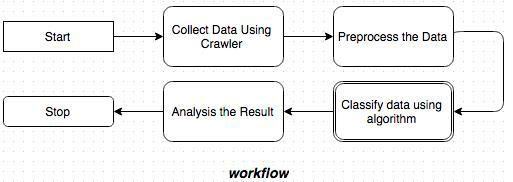
\includegraphics[scale=0.5]{images/fig-5.jpg}
\caption{Workflow}
\label{fig:x Workflow}
\end{figure}


\nomenclature{$\upsilon$}{Upsilon}
\nomenclature{$\epsilon$}{Epsilon}


% \chapter{First and Second}
% %\section{First and Second}
\section{Result Prediction based on First and Second Segment (Bat First)} 
As we have divided our total model into three segment and we actually consider first two segment for predicting the match outcome as we wanted to find out the final match result when match is in progress. We have taken total 91 match for making our model using multiple linear regression and we have merged all the attributes from those matches based on different segment. After analyzing those two segment our model has given 75\% accuracy. So, we can predict any match outcome when the match is in progress based on our model. As we did not take any attributes from the team who will bat second and considering the attribute which we got from first segment, our predicted model is quite good.

\begin{figure}[htbp]
\centering
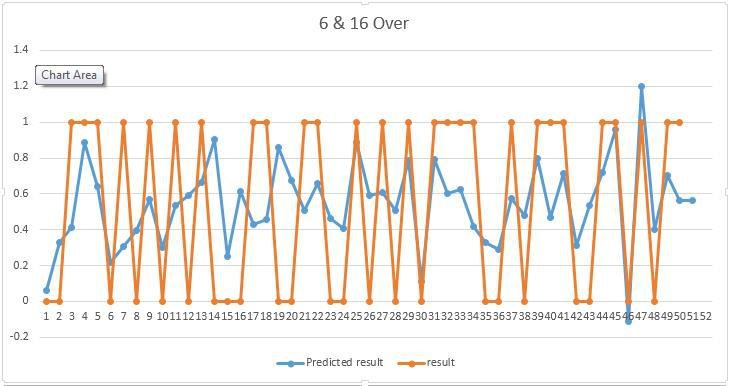
\includegraphics[scale=0.5]{images/fig-17.jpg}
\caption{First and Second Segment Prediction (Bat First)}
\label{fig:x First and Second Segment Prediction (Bat First)}
\end{figure}

From the figure above we can see the graph view of our model, here 0 means lost and 1 means win. So, if the predictive final value is less than 0.5 then the result would be consider as lose and if the predictive value is greater than 0.5 then it would be consider as win.

\textbf{Coefficient:} These are the coefficients values for all the attributes from Win prediction based on bat first.

\begin{table}[htbp]
\centering
\begin{tabular}{l | l}
Attributes & Coefficients\\
\hline
Intercept & 0.092219\\
Venue & 0.242112\\
M6ORN & 0.039573\\
M6OW & -0.12872\\
M16ORN & 0.05121\\
M16OW & -0.07214
\end{tabular}
\caption{First and Second Coefficient (Bat First)}
\label{tab:First and Second Coefficient (Bat First)}
\end{table}

\textbf{P-values:} These are the p values for all the at-tributes from Win prediction based on bat first.

\begin{table}[htbp]
\centering
\begin{tabular}{|l | r|}
\hline
Attributes & P-value\\
\hline
Intercept & 0.87596\\
\hline
Venue & 0.088577\\
\hline
M6ORN & 0.323375\\
\hline
M6OW & 0.084286\\
\hline
M16ORN & 0.246463\\
\hline
M16OW & 0.254117\\
\hline
\end{tabular}
\caption{First and Second Segment P-value (Bat First)}
\label{tab:First and Second Segment P-value (Bat First)}
\end{table}

\section{Result Prediction based on First and Second Segment (Bat Second)} 
While calculating for 2nd innings segments we get the run rate value from team batting first. Which makes a better impact on a prediction model and that time our model has given 85.5\% accuracy which is really good.

\begin{figure}[htbp]
\centering
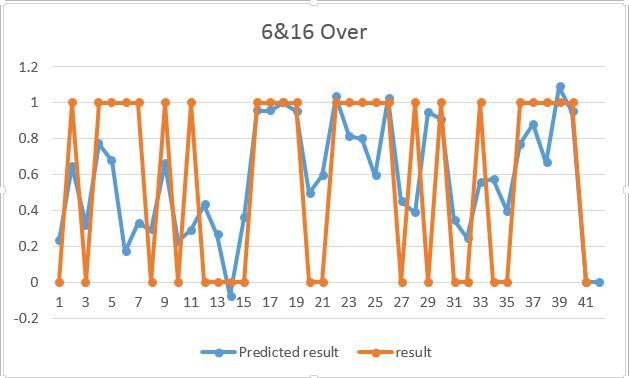
\includegraphics[scale=0.5]{images/fig-18.jpg}
\caption{First and Second Segment Run Prediction (Bat Second)}
\label{fig:x Frist and Second Segment Run Prediction (Bat Second)}
\end{figure}

\textbf{Coefficient:} These are the coefficients values for all the attributes from Win prediction based on bat second.
\vspace{3cm}

\begin{table}[htbp]
\centering
\begin{tabular}{|l | l|}
\hline
Attributes & Coefficients\\
\hline
Intercept & 2.282567\\
Venue & -0.04063\\
M6ORN & -0.02869\\
M6OW & -0.22694\\
M16ORN & -0.12705\\
M16OW & -0.10903\\
O6ORN & 0.008056\\
060W & 0.066748\\
O16ORN & 0.028731\\
O16OW & -0.0978\\
\hline
\end{tabular}
\caption{First and Second Segment Coefficient (Bat Second)}
\label{tab:First and Second Segment Coefficient (Bat Second)}
\end{table}

\textbf{P-values:} These are the p values for all the at-tributes from Win prediction based on bat second.

\setlength{\arrayrulewidth}{0.5mm}
\setlength{\tabcolsep}{12pt}
\renewcommand{\arraystretch}{1.5}

\begin{table}[ht]
\centering
\begin{tabular}{|l | l|}
\hline
\multicolumn{2}{| c |}{First and Second Segment P-value (Bat Second)} \\
\hline
Attributes & Coefficients\\
\hline
Intercept & 0.007165\\
Venue & 0.811504\\
M6ORN & 0.482433\\
M6OW & 0.019258\\
M16ORN & 0.112474\\
M16OW & 0.090761\\
O6ORN & 0.878555\\
060W & 0.429492\\
O16ORN & 0.633494\\
O16OW & 0.179298\\
\hline
\end{tabular}
\caption{First and Second Segment P-value (Bat Second)}
\label{tab:First and Second Segment P-value (Bat Second)}
\end{table}


\chapter{WorkPlan}
Our intention here is to elaborate on the ECG and EHR data available within the MEMIC-IV database, with special attention on the signal and text preprocessing techniques. To begin with, raw ECG signals are subjected to signal preprocessing which incorporates basic steps of noise filtering, physiological signals artificially removing the non-physiological interferences, data shaping into segments of manageable sizes, data scaling, and aligning the signals through re-referencing. On the other hand, the EHR which is usually in the prose format also undergoes text cleaning before being analyzed using text processing techniques involving conversion of uppercase letters to lowercase, segmenting or breaking down the text into the smallest possible words, eliminating auxiliary words and lemmatization or stemming which entails the reduction of a specific word to its base or root. To cope with the lack of data, i.e. introduce imputation, use resolving discrepancies between variable types, and adjust the length of data entries so that all data is the same length, by either cutting excess data or adding additional irrelevant data to the shorter entries. After data processing, ECG and EHR data are fused, and features a built on top of this data to extract informative attributes, for example, for training supervised machine learning, deep learning models, or reinforcement learning. The following steps include selecting a model, training this model, and adjusting hyperparameters for the chosen algorithm. The last stage consists of preparing the resulting model for deployment which enables its use for machine learning model usage to help identify outlying heart signals given the processed EHR and ECG data.
\vspace{0.5cm}


Here is the simple work flow chart given. 

\begin{figure}[ht]
\centering
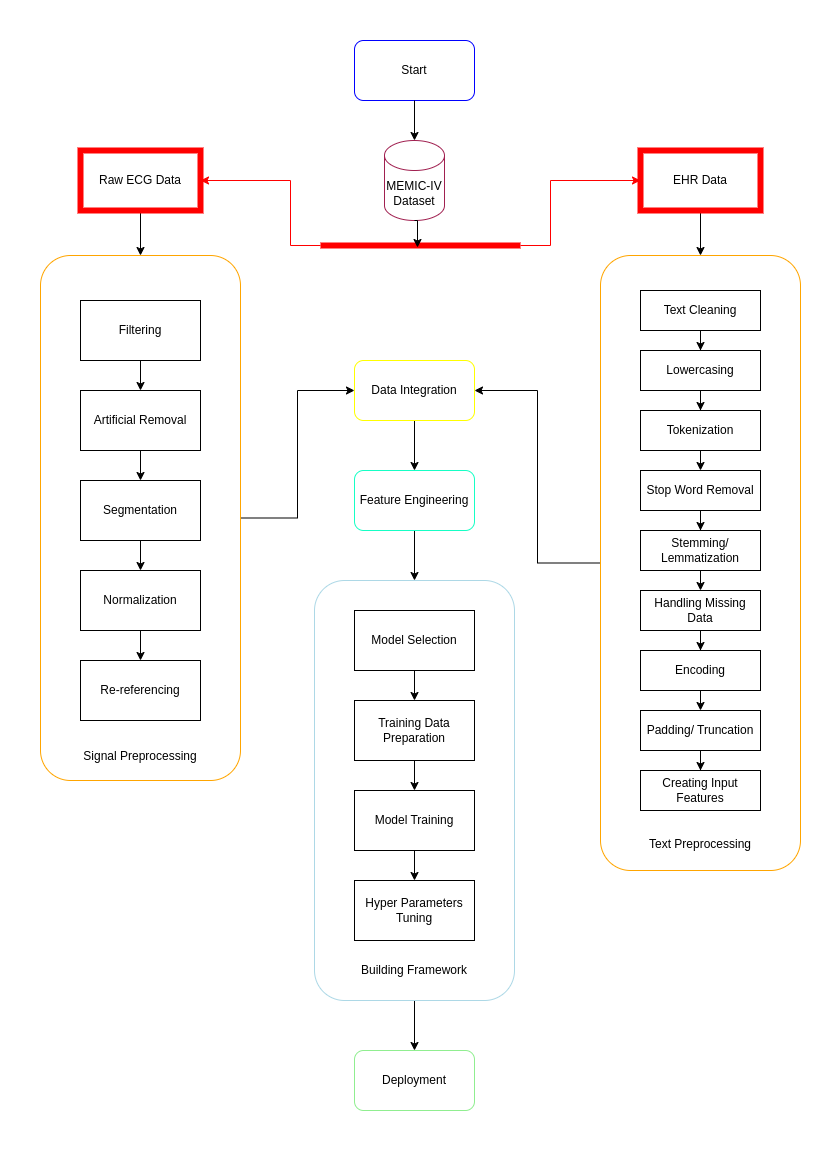
\includegraphics[scale=0.5]{images/workplan.png}
\caption{Workflow}
\label{fig:x Workflow}
\end{figure}

\chapter{Conclusion}
Since cardiovascular diseases are one of the leading causes of death in this age, it is crucial to identify cardiac risks early and accurately. Application of deep learning and natural language processing based algorithms in a large and diverse dataset can develop a good cardiac risk prediction model which can be able to predict more accurately and efficiently than previous models. That is why our study seeks to develop a system that can better predict cardiac risks by combining unstructured data from EHRs with ECG signals after applying our dual deep learning-based model to it. By merging these two data sets, we intend to develop a model that can enhance risk assessments' accuracy and comprehensibility. This study shows how Natural Language Processing(NLP)  and deep learning(DL) can work together to improve cardiac risk prediction and provide medical professionals with a vital tool.


\phantomsection
\printbibliography %Where the bibliography will be printed
\addcontentsline{toc}{chapter}{Bibliography}

% \chapter{Bibliography}
% \input{bibliography/references.tex}
% ********************************** Appendices ********************************
% %\begin{appendices} % Using appendices environment for more functionality
% \newpage
% \phantomsection
% \addcontentsline{toc}{chapter}{Appendix A How to install \LaTeX}
% % ******************************* Thesis Appendix A ****************************
\chapter*{How to install \LaTeX} 

\section*{Windows OS}

\subsection*{TeXLive package - full version}
\begin{enumerate}
\item	Download the TeXLive ISO (2.2GB) from\\
\href{https://www.tug.org/texlive/}{https://www.tug.org/texlive/}
\item	Download WinCDEmu (if you don't have a virtual drive) from \\
\href{http://wincdemu.sysprogs.org/download/}
{http://wincdemu.sysprogs.org/download/}
\item	To install Windows CD Emulator follow the instructions at\\
\href{http://wincdemu.sysprogs.org/tutorials/install/}
{http://wincdemu.sysprogs.org/tutorials/install/}
\item	Right click the iso and mount it using the WinCDEmu as shown in \\
\href{http://wincdemu.sysprogs.org/tutorials/mount/}{
http://wincdemu.sysprogs.org/tutorials/mount/}
\item	Open your virtual drive and run setup.pl
\end{enumerate}

or

\subsection*{Basic MikTeX - \TeX~ distribution}
\begin{enumerate}
\item	Download Basic-MiK\TeX (32bit or 64bit) from\\
\href{http://miktex.org/download}{http://miktex.org/download}
\item	Run the installer 
\item	To add a new package go to Start >> All Programs >> MikTex >> Maintenance (Admin) and choose Package Manager
\item	Select or search for packages to install
\end{enumerate}

\subsection*{TexStudio - \TeX~ editor}
\begin{enumerate}
\item	Download TexStudio from\\
\href{http://texstudio.sourceforge.net/\#downloads}
{http://texstudio.sourceforge.net/\#downloads} 
\item	Run the installer
\end{enumerate}

\section*{Mac OS X}
\subsection*{MacTeX - \TeX~ distribution}
\begin{enumerate}
\item	Download the file from\\
\href{https://www.tug.org/mactex/}{https://www.tug.org/mactex/}
\item	Extract and double click to run the installer. It does the entire configuration, sit back and relax.
\end{enumerate}

\subsection*{TexStudio - \TeX~ editor}
\begin{enumerate}
\item	Download TexStudio from\\
\href{http://texstudio.sourceforge.net/\#downloads}
{http://texstudio.sourceforge.net/\#downloads} 
\item	Extract and Start
\end{enumerate}


\section*{Unix/Linux}
\subsection*{TeXLive - \TeX~ distribution}
\subsubsection*{Getting the distribution:}
\begin{enumerate}
\item	TexLive can be downloaded from\\
\href{http://www.tug.org/texlive/acquire-netinstall.html}
{http://www.tug.org/texlive/acquire-netinstall.html}.
\item	TexLive is provided by most operating system you can use (rpm,apt-get or yum) to get TexLive distributions
\end{enumerate}

\subsubsection*{Installation}
\begin{enumerate}
\item	Mount the ISO file in the mnt directory
\begin{verbatim}
mount -t iso9660 -o ro,loop,noauto /your/texlive####.iso /mnt
\end{verbatim}

\item	Install wget on your OS (use rpm, apt-get or yum install)
\item	Run the installer script install-tl.
\begin{verbatim}
	cd /your/download/directory
	./install-tl
\end{verbatim}
\item	Enter command `i' for installation

\item	Post-Installation configuration:\\
\href{http://www.tug.org/texlive/doc/texlive-en/texlive-en.html\#x1-320003.4.1}
{http://www.tug.org/texlive/doc/texlive-en/texlive-en.html\#x1-320003.4.1} 
\item	Set the path for the directory of TexLive binaries in your .bashrc file
\end{enumerate}

\subsubsection*{For 32bit OS}
For Bourne-compatible shells such as bash, and using Intel x86 GNU/Linux and a default directory setup as an example, the file to edit might be \begin{verbatim}
edit $~/.bashrc file and add following lines
PATH=/usr/local/texlive/2011/bin/i386-linux:$PATH; 
export PATH 
MANPATH=/usr/local/texlive/2011/texmf/doc/man:$MANPATH;
export MANPATH 
INFOPATH=/usr/local/texlive/2011/texmf/doc/info:$INFOPATH;
export INFOPATH
\end{verbatim}
\subsubsection*{For 64bit OS}
\begin{verbatim}
edit $~/.bashrc file and add following lines
PATH=/usr/local/texlive/2011/bin/x86_64-linux:$PATH;
export PATH 
MANPATH=/usr/local/texlive/2011/texmf/doc/man:$MANPATH;
export MANPATH 
INFOPATH=/usr/local/texlive/2011/texmf/doc/info:$INFOPATH;
export INFOPATH

\end{verbatim}



%\subsection{Installing directly using Linux packages} 
\subsubsection*{Fedora/RedHat/CentOS:}
\begin{verbatim} 
sudo yum install texlive 
sudo yum install psutils 
\end{verbatim}


\subsubsection*{SUSE:}
\begin{verbatim}
sudo zypper install texlive
\end{verbatim}


\subsubsection*{Debian/Ubuntu:}
\begin{verbatim} 
sudo apt-get install texlive texlive-latex-extra 
sudo apt-get install psutils
\end{verbatim}


% \newpage
% \phantomsection
% \addcontentsline{toc}{chapter}{Appendix B Overleaf: GitHub for \LaTeX\ projects}
% % ******************************* Thesis Appendix B ********************************

\chapter*{Overleaf: GitHub for \LaTeX\ projects }

This Project was developed using Overleaf(\url{https://www.overleaf.com/}), an online \LaTeX\ editor that allows real-time collaboration and online compiling of projects to PDF format. In comparison to other \LaTeX\ editors, Overleaf is a server-based application, which is accessed through a web browser.




% %\end{appendices}

\end{document}